\documentclass[10pt,a4paper]{article}
\usepackage[a4paper,margin=1.8cm]{geometry}
\usepackage[T1]{fontenc}
\usepackage{lmodern}
\usepackage{microtype}
\usepackage{booktabs}
\usepackage{tabularx}
\usepackage{array}
\usepackage[table]{xcolor}
\usepackage{enumitem}
\usepackage{titlesec}
\usepackage{url}
\usepackage[colorlinks=true,linkcolor=blue!50!black,urlcolor=blue!50!black]{hyperref}
\usepackage{graphicx}
\setlength{\textfloatsep}{1.6ex plus 0.6ex}
\setlength{\floatsep}{1.4ex plus 0.6ex}
\renewcommand{\topfraction}{0.9}
\renewcommand{\textfraction}{0.08}
\renewcommand{\floatpagefraction}{0.85}
\newcommand{\figcap}[1]{\caption{\footnotesize #1}}
\setlist{nosep,leftmargin=1.3em}
\titlespacing*{\section}{0pt}{1.4ex}{0.6ex}
\setlength{\parindent}{0pt}
\setlength{\parskip}{0.55ex}
\renewcommand{\arraystretch}{1.12}
\newcommand{\iss}[1]{\href{https://github.com/JieGH/RVV_code_gen_via_MLIR_xDSL/issues/#1}{\##1}}
\newcommand{\good}[1]{\textcolor{green!45!black}{\textbf{#1}}}
\newcommand{\bad}[1]{\textcolor{red!70!black}{\textbf{#1}}}
\newcommand{\key}[1]{\textbf{\textcolor{blue!55!black}{#1}}}
\newcommand{\callout}[1]{\fcolorbox{blue!50!black}{blue!4}{\parbox{0.96\textwidth}{#1}}}
\titleformat{\section}{\large\bfseries}{\thesection}{0.6em}{}

\graphicspath{{issue-54-figs/simple/en/}}
\title{\vspace{-1.2cm}\textbf{One column at a time}\\[2pt]\large The issue \iss{54} fix, in plain words: what changes in the code and why it helps}
\author{RVV\_code\_gen\_via\_MLIR\_xDSL, \texttt{pure-xdsl}; SpacemiT X60 (RVV 1.0, VLEN 256)}
\date{29 October 2026. Short guide; the full report is \texttt{issue-54-brief.pdf}}
\begin{document}
\maketitle\vspace{-1.5ex}

\callout{
\textbf{The problem.} Our B3 benchmark often falls into a \emph{slow state}: about 4.6 GOPs instead of 7.0. The B packer sets it off, because it
reads B in a pattern that the cache hardware handles badly.\\[3pt]
\textbf{The fix.} \key{Read B one column at a time, 32 numbers per load, then write those numbers into their places in Bc.}\\[3pt]
\textbf{The result.} Our design goes from 4.63 to 7.03 GOPs, and Adri\'an's reference design from 4.49 to 7.14 GOPs with the same fix.
\key{Bc comes out byte for byte the same, so the answers cannot change.}}

\section{What the packer does}
B is stored column by column. The numbers of one column sit next to each other in memory; the next column starts $K\times4$ bytes
later (\texttt{ldb*4} = 1536 B for $K=384$). The packer copies B into a buffer called Bc, in the order the microkernel will read it. It is
only a copy: it does no arithmetic.

\section{Current way and the fix}
\begin{figure}[!ht]
\centering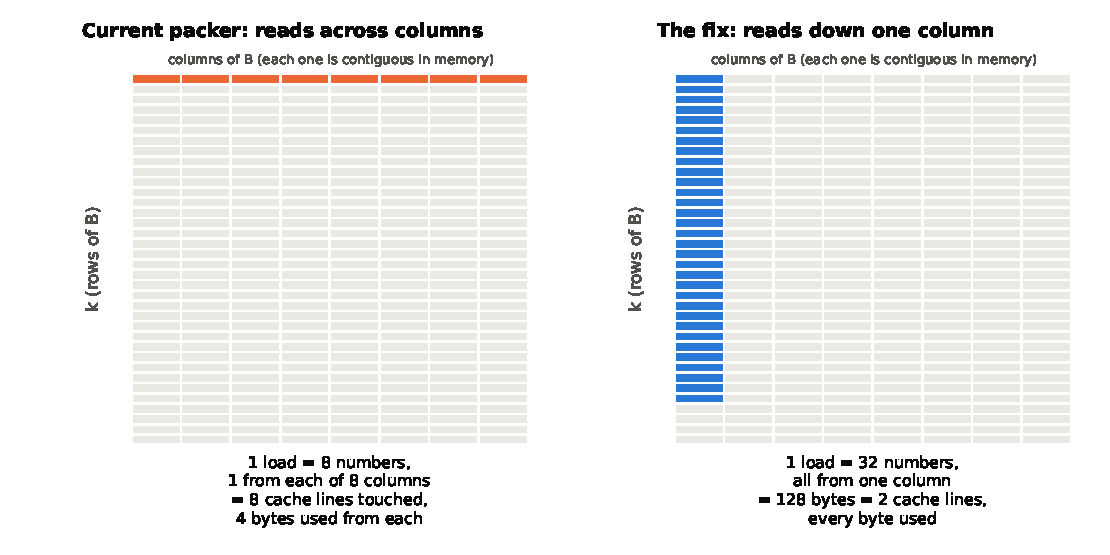
\includegraphics[width=0.8\textwidth]{fig_simple_read.pdf}
\figcap{B drawn as 8 columns of 36 values (one small box is one fp32 number). Coloured boxes are the numbers one vector load reads.}
\end{figure}
\begin{itemize}
\item \textbf{Current packer.} Each load takes 1 number from each of 8 columns. \key{That touches 8 different cache lines and uses only 4 bytes
  of each 64-byte line}, and the next load starts again 1536 B away from the last one. The L1D prefetcher then becomes less effective, and
  pack and compute both slow down.
\item \textbf{The fix.} Each load takes 32 numbers from one column. \key{That is 128 B in a row: 2 cache lines, every byte used}, and the next
  load continues straight after it. This is the access order that prefetchers are built for.
\item \textbf{Where the jump went.} The jump is still needed, because Bc is laid out by rows of $k$. We moved it from the load to the
  \emph{store}: loads from the big matrix B are now in order, and the strided store writes into Bc.
\end{itemize}

\section{What changes in the intrinsics}
Only three calls change. \texttt{e32} means 32-bit elements (fp32); \texttt{m1} and \texttt{m4} are the LMUL, how many vector registers
one instruction uses.
\begin{center}\footnotesize
\begin{tabular}{@{}p{1.6cm}p{4.7cm}p{5.2cm}p{4.4cm}@{}}
\toprule
 & current packer & the fix & what it means \\
\midrule
length & \texttt{vsetvl\_e32m1} & \texttt{vsetvl\_e32m4} & up to 8 numbers $\to$ up to 32 \\
load & \texttt{vlse32\_v\_f32m1(src, ldb*4, vl)} & \texttt{vle32\_v\_f32m4(src, vl)} & strided across columns $\to$ plain, in order \\
store & \texttt{vse32\_v\_f32m1(dst, v, vl)} & \texttt{vsse32\_v\_f32m4(dst, RR*4, v, vl)} & 8 side by side $\to$ one per row of Bc \\
\bottomrule
\end{tabular}
\end{center}
The same code for the fix, as it is in the reference design's \texttt{pack\_CB} (the \texttt{if} guarding the vector path is left out), and the RISC-V
instructions it becomes:
{\footnotesize\begin{verbatim}
size_t vl = __riscv_vsetvl_e32m4((size_t) len);              // len is at most 32
vfloat32m4_t v = __riscv_vle32_v_f32m4(src, vl);             // 32 numbers down one column of B
__riscv_vsse32_v_f32m4(dst, (ptrdiff_t) RR * 4, v, vl);      // one number per row of Bc

current:   vsetvli zero,a7,e32,m1,ta,ma
           vlse32.v v24,(a4),t1  (t1 = 1536 B)
the fix:   vsetvli t4,t4,e32,m4,ta,ma
           vle32.v  v24,(a3)
           vsse32.v v24,(s6),a5  (a5 = RR*4)
\end{verbatim}}
\begin{figure}[!ht]
\centering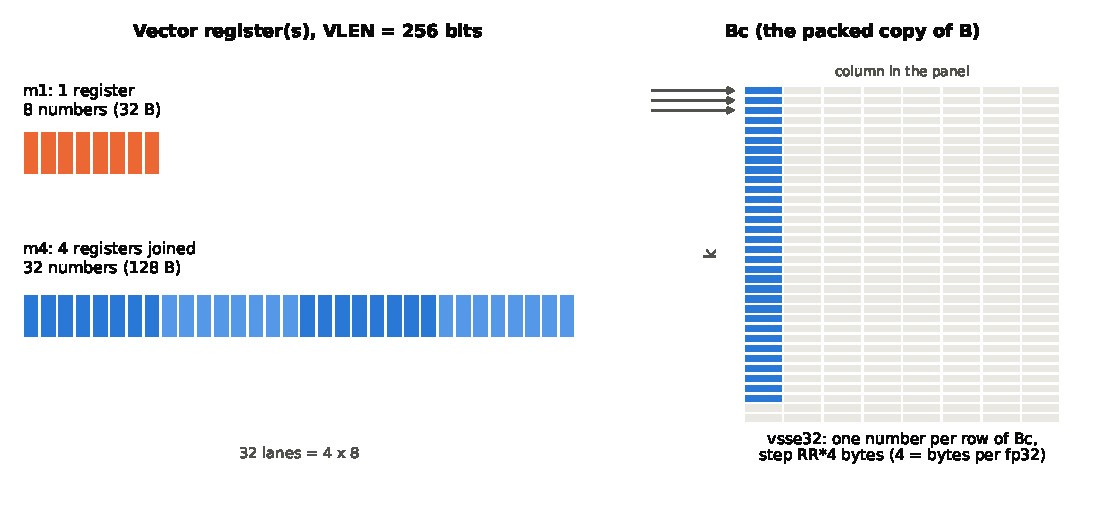
\includegraphics[width=0.9\textwidth]{fig_simple_lmul_store.pdf}
\figcap{Left: one \texttt{m1} register holds 8 numbers; \texttt{m4} joins 4 of them into 32. Right: the 32 numbers from one column of B go
into one column of Bc, one number per row.}
\end{figure}

\callout{\textbf{Two different 4s.} In \texttt{ldb*4} and \texttt{RR*4}, the 4 is the \emph{bytes in one fp32 number}, because the intrinsics take
strides in bytes. In \texttt{m4}, the 4 is \emph{how many registers are joined}: $4\times8=32$ numbers.}

\section{Why the result cannot change}
A packer only copies. Both versions put every number of B at the same place in Bc, \texttt{Bc[p*NR*kc + k*NR + j]}; only the order of
the copying differs. We checked this byte for byte on the host for the reference design's patched packer (1008 cases), and the microkernel,
blocking and Bc layout are untouched.

\section{Result}
\begin{figure}[!ht]
\centering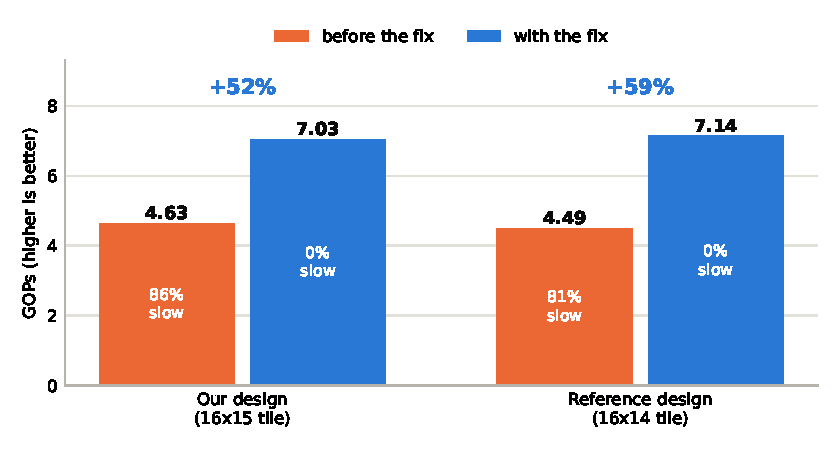
\includegraphics[width=0.62\textwidth]{fig_simple_result.pdf}
\figcap{B3 (64$\times$384$\times$384), uninstrumented build, reference protocol, core 4. Our design: series 1, 22 October. Reference design:
29 October, 3 launches (4.39--4.60 $\to$ 7.11--7.18). Text in the bars: share of slow reps.}
\end{figure}
\key{The fix removes the slow state in both designs}: 86\% and 81\% slow reps become 0\%.

\section{Is it worth it?}
A simpler choice is the scalar packer that the generator already has (\texttt{use\_scalar\_pack}). It helps, but it is not safe everywhere:
38\% slow reps on B3 at the default tile, 4.64 GOPs on B3\_K256 at 16$\times$15, and 3--4\% lower on B2. \key{The fix is the best, or within 1\% of the best, in
11 of 12 cells.} What we do not know yet is how much of a real model's time is in small-M, large-K layers like B3; that decides how much the
fix is worth overall.

\section{Likely questions}
\textbf{Why not just transpose B first?} A transpose is an extra copy of the whole matrix, and Bc still has to be built after it. \key{The fix
does the transpose inside the packing step, in the same single pass}: no extra copy, and the GEMM is called as before.

\textbf{Does reading in a different order change the result?} No. A packer only copies, and every number lands at the same address of Bc as before
(Bc is byte for byte the same). Only the order of the copying differs.

\textbf{Does it make packing slower?} A little, in a fast rep: the pack-only mean at 16$\times$15 on B3 is 0.8218 ms against 0.6443 ms for the
current vector packer. But \key{it never turns slow}, while the current packer spends 91\% of its reps at 1.1994 ms. It also needs fewer
instructions: 60 loads per panel instead of 256 (B3, default tile).

\textbf{Why does it happen on B3 and not everywhere?} Not fully explained. The step between the 8 columns (1536 B at $K=384$) matters, and padding
\texttt{ldb} changes the state, but in no simple pattern (\iss{49}). Smaller tiles avoid it in some cells (B3 at 16$\times$6) and not in others
(B3 at 16$\times$8: 3.83 GOPs).

\textbf{Is this only my design, or the reference design too?} Both. The reference packs B in the same order, one number per load with the same
1536 B step, and on B3 at 16$\times$14 it was 81\% slow (4.49 GOPs). The reference developer sees no flaw in the packing code itself, which fits:
the result is correct, and only the speed suffers.

\textbf{Did my vector packer make it worse?} In most cells, yes. At the default tile it is 86\% slow, against 38\% for the scalar packer.
Going back to scalar does not remove the slow state either.

\textbf{Why \texttt{m4} and not \texttt{m1}?} The \texttt{m1} version of the same idea (\texttt{col-g1}) is also never slow. \texttt{m4} was chosen
because one load then covers 2 whole cache lines and needs fewer instructions. A packer only copies, so using 4 of the 32 registers
per group costs nothing.

\textbf{Would a smaller tile, or padding the matrix, be enough?} Not reliably, as above: both change the state in no simple pattern, while the
fix gave no slow rep in any of the 18 cells we ran.

\textbf{How far do the reference numbers go?} Only B3, at two tiles. At 16$\times$14 it went from 4.49 to 7.14 GOPs; at 16$\times$16 from 4.20 to
4.41, a much smaller gain, so other effects remain there. Our design was run on 18 GEMM cells.

\textbf{Did you change Adri\'an's repository?} No. A script, \texttt{ref\_pack\_fix.py}, applies the fix to a staged copy of the reference source (the file \texttt{gemm\_blis.c}), so
the files under \texttt{ext/} are untouched.
\end{document}
